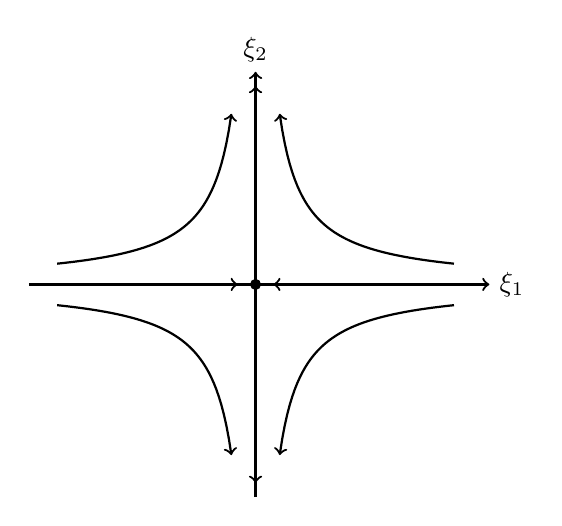
\begin{tikzpicture}[x=0.9cm,y=0.9cm,thick]
  \draw[->] (-3.2,0)--(3.3,0) node[right] {$\xi_1$};
  \draw[->] (0,-3.0)--(0,3.0) node[above] {$\xi_2$};
  % Stable horizontal and unstable vertical separatrices.
  \draw[->] (-2.8,0)--(-0.25,0); \draw[->] (2.8,0)--(0.25,0);
  \draw[->] (0,0.25)--(0,2.8); \draw[->] (0,-0.25)--(0,-2.8);
  % Hyperbolas: forward motion goes from the stable direction toward the unstable one.
  \foreach \sx in {-1,1} {\foreach \sy in {-1,1} {
    \draw[->] plot[domain=2.8:0.34,samples=70,variable=\s]
      ({\sx*\s},{\sy*0.82/\s});
  }}
  \fill (0,0) circle (2pt);
\end{tikzpicture}
